%! Author = sbbfti
%! Date = 10/06/2020

%% Use the option review to obtain double line spacing
%% \documentclass[preprint,review,12pt]{elsarticle}

%% Use the options 1p,twocolumn; 3p; 3p,twocolumn; 5p; or 5p,twocolumn
%% for a journal layout:
%% \documentclass[final,1p,times]{elsarticle}
\documentclass[final,1p,times,twocolumn]{elsarticle}
%% \documentclass[final,3p,times]{elsarticle}
%% \documentclass[final,3p,times,twocolumn]{elsarticle}
%% \documentclass[final,5p,times]{elsarticle}
%% \documentclass[final,5p,times,twocolumn]{elsarticle}

%% \documentclass[review, 1p]{elsarticle}

\usepackage{mypreamble}
\usepackage{setspace}

\usepackage[nonumberlist,nogroupskip]{glossaries}

\newglossaryentry{7730}
{
name={ISO~7730:2005},
description={ISO~7730:2005 is a thermal comfort standard developed by ISO}
}

\newglossaryentry{55}
{
name={ASHRAE~55--2020},
description={ASHRAE~55--2020 is a thermal comfort standard developed by ANSI and ASHRAE}
}

\makenoidxglossaries


\begin{document}

    \begin{frontmatter}

    \title{Graph Attention Network (GAT) based Branching in
Combinatorial Optimization Problems}

    \author[label1]{Gökhan Murali\corref{mycorrespondingauthor}}
    \ead{gmurali21@ku.edu.tr}
    \author[label1]{Prof. Metin Türkay}

    \affiliation[label1]{organization={Koc University},
             addressline={Rumelifeneri Yolu, Sariyer},
             city={Istanbul},
             postcode={34450},
             %state={NSW},
             country={Turkiye}}

    \cortext[mycorrespondingauthor]{Corresponding author}

    \begin{abstract}


        In this study, the main aim is to imitate the Strong Branching strategy during the branching phase, which is one of the most critical components of the Branch \& Bound algorithm used for solving Combinatorial Optimization problems, by implementing a Graph Attention Network (GAT)-based method.
        Strong Branching is an effective strategy in terms of the number of nodes, keeping the search tree short.
        However, it is highly time consuming because it solves the linear programming problem twice for each branching candidate variable at each node.
        To eliminate the time cost of the Strong Branching strategy, this study attempts to learn a function implementing the GAT technique that can make Strong Branching-like decisions in a shorter time.

        In the literature, there are studies that successfully imitate the Strong Branching strategy using Graph Convolutional Neural Network (GCNN). In the GCNN method, all neighbouring nodes have the same importance for a node.
        In contrast, the GAT  architecture allows neighbouring nodes to have different levels of importance for a node.
        Therefore, it is hypothesized that GAT-based methods will yield better results.

        Experiments conducted in this study have shown that the GAT architecture provides decisions closer to the Strong Branching strategy compared to the GCNN architecture.
        GAT-based methods enable problems to be solved with fewer nodes compared to GCNN.
        In summary, GAT is a promising tool for imitating the effective yet slow Strong Branching strategy.
        Supplementary code for this study can be found at \url{https://github.com/GokhanMurali/learn2branchbyGAT}.
    \end{abstract}


    \begin{keyword}
        Mixed Integer Programming \sep Branch \& Bound \sep Strong Branching \sep Machine Learning \sep Neural Networks \sep Graph Neural Network (GNN) \sep Convolution \sep Message Passing \sep Graph Attention Network (GAT) \sep Graph Convolutional Neural Network (GCNN)
    \end{keyword}

\end{frontmatter}


    %%! Author = federico
%! Date = 10/06/2020

\section*{Nomenclature}
\renewcommand{\baselinestretch}{0.75}\normalsize
\renewcommand{\aclabelfont}[1]{\textsc{\acsfont{#1}}}
\begin{acronym}[longest]

    \acro{t-db}[$t_{db}$]{dry-bulb air temperature\acroextra{, $^{\circ}$C}}
    \acro{t-wb}[$t_{wb}$]{wet-bulb air temperature\acroextra{, $^{\circ}$C}}
    \acro{ti}[$t_{i}$]{indoor air temperature\acroextra{, $^{\circ}$C}}
    \acro{tout}[$t_{out}$]{outdoor air temperature\acroextra{, $^{\circ}$C}}
    \acro{t-op}[$t_{o}$]{operative air temperature\acroextra{, $^{\circ}$C}}
    \acro{t-cl}[$t_{cl}$]{clothing temperature\acroextra{, $^{\circ}$C}}
    \acro{tg}[$t_{g}$]{globe temperature\acroextra{, $^{\circ}$C}}
    \acro{rh}[$RH$]{relative humidity\acroextra{, \%}}
    \acro{v}[$V$]{average air speed\acroextra{, m/s}}
    \acro{t-r}[$\overline{t_{r}}$]{mean radiant temperature\acroextra{, $^{\circ}$C}}
    \acro{clo}[$I_{cl}$]{total clothing insulation\acroextra{, clo}}
    \acro{i-cl}[$i_{cl}$]{permeation efficiency of water vapor through the clothing layer}
    \acro{met}[$M$]{rate of metabolic heat production\acroextra{, W/m\textsuperscript{2}}}
    \acro{work}[$W$]{rate of mechanical work accomplished\acroextra{, W/m\textsuperscript{2}}}
    \acro{t-sk}[$t_{sk}$]{skin mean temperature\acroextra{, $^{\circ}$C}}
    \acro{t-sk-n}[$t_{sk,n}$]{neutral skin mean temperature\acroextra{, $^{\circ}$C}}
    \acro{t-cr}[$t_{cr}$]{core mean temperature\acroextra{, $^{\circ}$C}}
    \acro{t-re}[$t_{re}$]{rectal temperature\acroextra{, $^{\circ}$C}}
    \acro{t-cr-n}[$t_{cr,n}$]{neutral core mean temperature\acroextra{, $^{\circ}$C}}
    \acro{r-cl}[$R_{cl}$]{thermal resistance of clothing\acroextra{, m\textsuperscript{2}K/W}}
    \acro{r-e-cl}[$R_{e,cl}$]{evaporative heat transfer resistance of clothing layer\acroextra{, m\textsuperscript{2}kPa/W}}
    \acro{f-cl}[$f_{cl}$]{clothing area factor $A_{cl}/A_{body}$\acroextra{, m\textsuperscript{2}K/W}}
    \acro{h}[$h$]{sum of convective $h_{c}$ and radiative $h_{r}$ heat transfer coefficients\acroextra{, W/(m\textsuperscript{2}K)}}
    \acro{h-r}[$h_{r}$]{linear radiative heat transfer coefficient\acroextra{, W/(m\textsuperscript{2}K)}}
    \acro{h-c}[$h_{c}$]{convective heat transfer coefficient\acroextra{, W/(m\textsuperscript{2}K)}}
    \acro{h-e}[$h_{e}$]{evaporative heat transfer coefficient\acroextra{, W/(m\textsuperscript{2}kPa)}}
    \acro{a}[$\alpha$]{fraction of the total body mass considered
to be thermally in the skin compartment}

    \acro{cl-a}[$A_{cl}$]{clothing surface area\acroextra{, m\textsuperscript{2}}}

    \acro{e}[$\varepsilon$]{average emissivity of clothing or body surface}
    \acro{sigma}[$\sigma$]{Stefan-Boltzmann constant\acroextra{, 5.67 x 10\textsuperscript{-8} W/(m\textsuperscript{2}K\textsuperscript{2})}}

    \acro{a-r}[$A_{r}$]{effective  radiation  area  of  the  body\acroextra{, m\textsuperscript{2}}}
    \acro{body-a}[$A_{body}$]{body surface area\acroextra{, m\textsuperscript{2}}}
    \acro{body-w}[$mass$]{body mass\acroextra{, kg}}
    \acro{body-h}[$height$]{body height\acroextra{, m}}

    \acro{pmv}[PMV]{Predicted Mean Vote}
    \acro{ppd}[PPD]{Predicted Percentage of Dissatisfied\acroextra{, \%}}
    \acro{set}[SET]{Standard Effective Temperature\acroextra{, $^{\circ}$C}}
    \acro{ce}[CE]{Cooling Effect\acroextra{, $^{\circ}$C}}
    \acro{phs}[PHS]{Predicted Heat Strain}

    \acro{BMS}[BMS]{Building Management System}
    \acro{HVAC}[HVAC]{Heating, Ventilation, and Air Conditioning}
    \acro{VAV}[VAV]{Variable Air Volume}
    \acro{AHU}[AHU]{Air Handling Unit}

    \acro{ema}[EMA]{Ecological Momentary Assessment}
    \acro{sdk}[SDK]{Software Development Kit}
    \acro{api}[API]{Application Programming Interface}

    \acro{s-cr}[$S_{cr}$]{rate of heat storage in the core compartment\acroextra{, W/m\textsuperscript{2}}}
    \acro{s-sk}[$S_{sk}$]{rate of heat storage in the skin compartment\acroextra{, W/m\textsuperscript{2}}}
    \acro{s}[$S$]{rate of heat storage in the human body\acroextra{, W/m\textsuperscript{2}}}
    \acro{e-res}[$E_{res}$]{rate of evaporative heat loss from respiration\acroextra{, W/m\textsuperscript{2}}}
    \acro{e-dif}[$E_{dif}$]{rate of evaporative heat loss from moisture diffused through the skin\acroextra{, W/m\textsuperscript{2}}}
    \acro{e-rsw}[$E_{rsw}$]{rate of evaporative heat loss from sweat evaporation\acroextra{, W/m\textsuperscript{2}}}
    \acro{e-sk}[$E_{sk}$]{total rate of evaporative heat loss from skin\acroextra{, W/m\textsuperscript{2}}}
    \acro{e-max}[$E_{max}$]{maximum rate of evaporative heat loss from skin\acroextra{, W/m\textsuperscript{2}}}
    \acro{c-res}[$C_{res}$]{rate of convective heat loss from respiration\acroextra{, W/m\textsuperscript{2}}}
    \acro{c-r}[$C + R$]{sensible heat loss from skin\acroextra{, W/m\textsuperscript{2}}}
    \acro{q-res}[$q_{res}$]{total rate of heat loss through respiration\acroextra{, W/m\textsuperscript{2}}}
    \acro{q-sk}[$q_{sk}$]{total rate of heat loss from skin\acroextra{, W/m\textsuperscript{2}}}
    \acro{w}[$w$]{skin wettedness}
    \acro{w-max}[$w_{max}$]{skin wettedness practical upper limit}
    \acro{m-sweat}[$m_{rsw}$]{rate at which regulatory sweat is generated\acroextra{, mL/h\textsuperscript{2}}}
    \acro{m-bl}[$m_{bl}$]{skin blood flow\acroextra{, L/(hm\textsuperscript{2})}}
    \acro{c-sw}[$c_{sw}$]{driving coefficient for regulatory sweating\acroextra{, g/(hKm\textsuperscript{2})}}

    \acro{p-sk}[$p_{sk,s}$]{water vapor pressure at skin\acroextra{, kPa}}
    \acro{p-a}[$p_{a}$]{water vapor pressure in ambient air\acroextra{, kPa}}

    \acro{wmo}[WMO]{World Meteorological Organization}
    \acro{who}[WHO]{World Health Organization}
    \acro{cdc}[CDC]{Centers for Disease Control and Prevention}
    \acro{noaa}[NOAA]{National Oceanic and Atmospheric Administration}
    \acro{epa}[EPA]{United States Environmental Protection Agency}
    \acro{iea}[IEA]{International Energy Agency}
    \acro{un}[UN]{United Nations}

\end{acronym}
\renewcommand{\baselinestretch}{1}\normalsize


    %\doublespacing

    %% The lineno packages adds line numbers. Start line numbering with
    %% \begin{linenumbers}, end it with \end{linenumbers}. Or switch it on
    %% for the whole article with \linenumbers.
    %% \usepackage{lineno}

    \linenumbers

    \acresetall

    \section{Introduction}\label{sec:introduction}

If you are new to \LaTeX{}, you can check my YouTube video \href{https://youtu.be/CjuYkcA35dw}{\LaTeX{} Masterclass}.

If you are in a hurry, you can check my YouTube video \href{https://youtu.be/g0YdIs4oJm8}{Introduction to \LaTeX{}}.

\subsection{How to cite a paper}\label{subsec:how-to-cite-a-paper}
This is an example on how to cite a paper~\cite{Tartarini2020a}.

\subsection{How to add acronyms/nomenclature}\label{subsec:how-to-add-acronyms}
This is an example on how to add acronyms.
You can reference the acronym using the command \verb!\ac{t-db}! this will result in the following \ac{t-db}.
If you use the command \verb!\ac{t-db}! again, it will result in \ac{t-db}.
You can check the list of acronyms in the \texttt{myacronyms.tex} file.

\subsection{Glossary}\label{subsec:glossary}

This is an example on how to add a glossary.
You can reference the glossary using the command \verb!\gls{7730}! this will result in the following \gls{7730}.
You can check the list of glossary terms in the \texttt{myglossary.tex} file.

\subsection{How to add a table}\label{subsec:how-to-add-a-table}
This is an example on how to add a table.
The table is shown in Table~\ref{tab:example}.

\begin{table}[htb!]
    \centering
    \begin{tabular}{|c|c|}
        \hline
        \textbf{Column 1} & \textbf{Column 2} \\
        \hline
        Row 1 & Value 1 \\
        Row 2 & Value 2 \\
        Row 3 & Value 3 \\
        \hline
    \end{tabular}
    \caption{This is an example table.}
    \label{tab:example}
\end{table}

\subsection{How to add a figure}\label{subsec:how-to-add-a-figure}
This is an example on how to add a figure.
The figure is shown in Figure~\ref{fig:example}.

\begin{figure}[htb!]
    \centering
    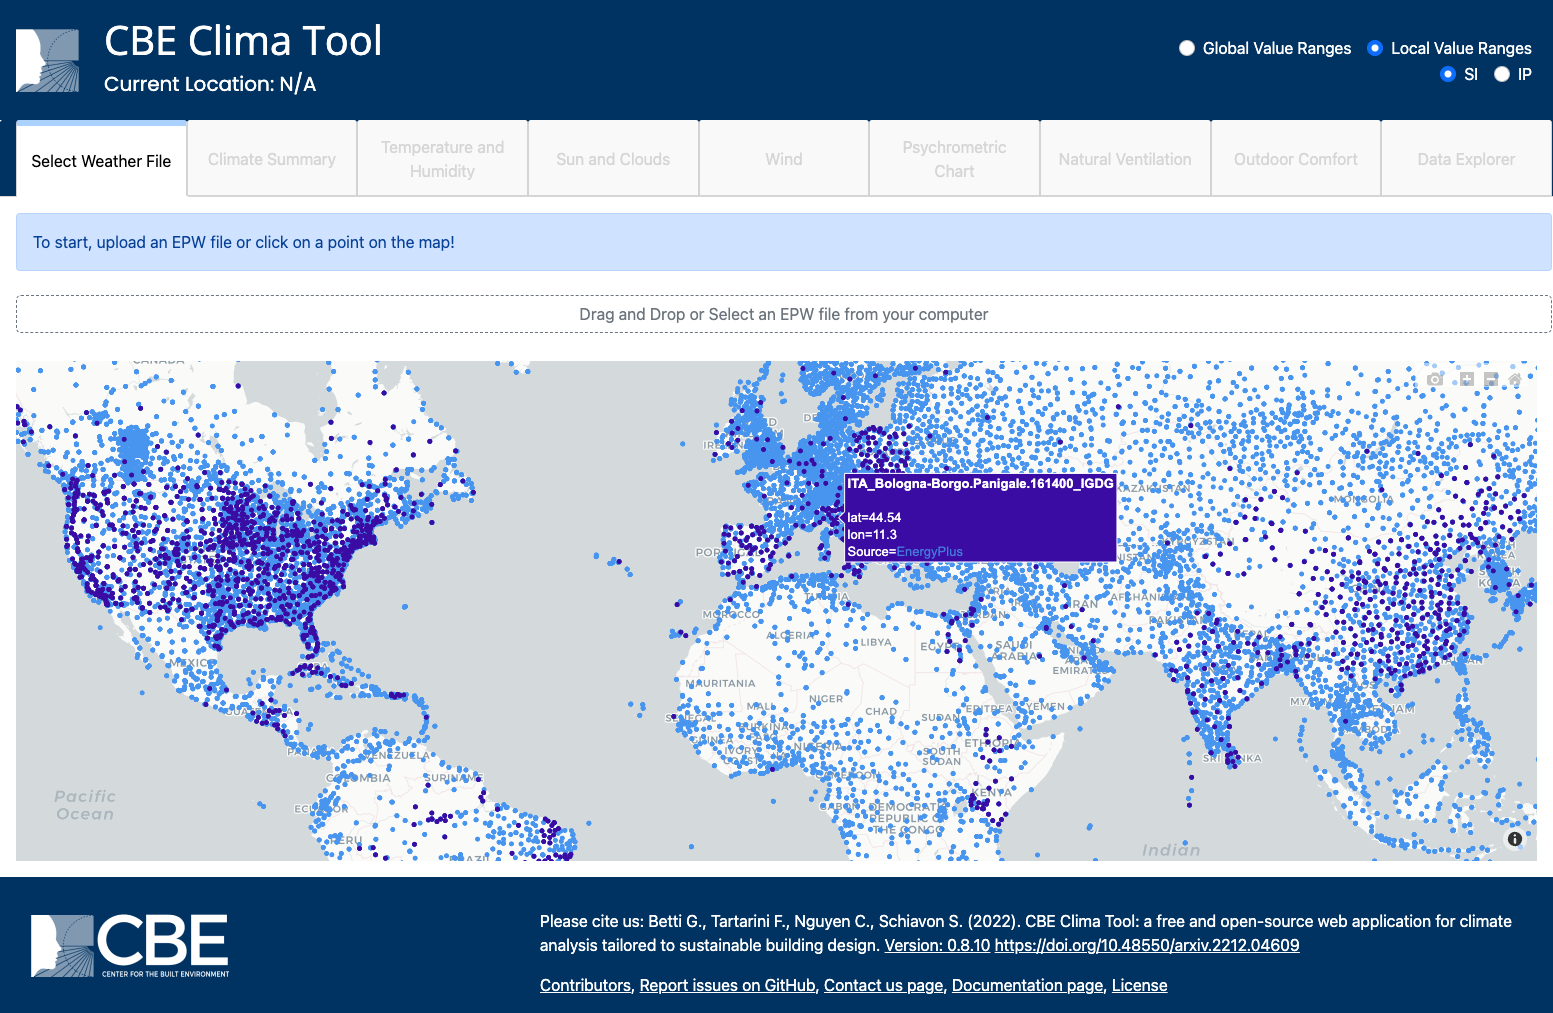
\includegraphics[width=0.75\textwidth]{figures/example_clima}
    \caption{This is an example figure.}
    \label{fig:example}
\end{figure}

\subsection{How to write numbers}\label{subsec:how-to-write-numbers}
This is an example on how to write numbers.

\subsection{How to import a variable}\label{subsec:how-to-import-a-variable}
This is an example on how to import a variable.
You can import a variable using the command \verb!\var{example_variable}! this will result in the following \var{example_variable}.
You can check the list of variables in the \texttt{mydata.tex} file.
If you want to find out more on how to import variables, you can check my YouTube video \href{https://ctan.org/pkg/datatool}{datatool} package documentation.

    \section{Methodology}\label{sec:methodology}

    \section{Results}\label{sec:results}

    \section{Conclusions}\label{sec:conclusions}


    \clearpage

    \bibliography{mybibfile}

    \clearpage

    \appendix

\section{Appendix}\label{sec:appendix}


\end{document}